\documentclass[10pt]{article}
\usepackage[utf8]{inputenc}
\usepackage[T1]{fontenc}
\usepackage{amsmath}
\usepackage{amsfonts}
\usepackage{amssymb}
\usepackage[version=4]{mhchem}
\usepackage{stmaryrd}
\usepackage{hyperref}
\usepackage{graphicx}
\usepackage{enumitem}
\usepackage{multirow}
\graphicspath{ {./CS-234/} }

\title{Assignment 2 - DFAs and Propositional Logic}

\author{CS 234}
\date{Daniel Lee}


\begin{document}
\maketitle

\section*{1 \quad DFAs and Propositional Logic on Paper}

\begin{enumerate}[label={}]
      \item Give the full 5-tuple for DFAs for the following languages:


            2.2. $\left\{w \in\{0,1\}^*: w\right.$ ends with a 1$\}$

            $\left(\left\{q_0, q_1\right\},\{0,1\}, \delta, q_0,\left\{q_1\right\}\right)$


            \begin{tabular}{ |c|c|c|  }
                  \hline
                  $\delta$ & $0$   & $1$   \\
                  \hline
                  $q_0$    & $q_0$ & $q_1$ \\
                  $q_1$    & $q_0$ & $q_1$ \\
                  \hline
            \end{tabular}


            2.4. $\left\{w \in\{0,1\}^*: w\right.$ has 01 as a substring $\}$

            $\left(\left\{q_0, q_1, q_2\right\},\{0,1\}, \delta, q_0,\left\{q_2\right\}\right)$

            \begin{tabular}{ |c|c|c|  }
                  \hline
                  $\delta$ & $0$   & $1$   \\
                  \hline
                  $q_0$    & $q_1$ & $q_0$ \\
                  $q_1$    & $q_1$ & $q_2$ \\
                  $q_2$    & $q_2$ & $q_2$ \\
                  \hline
            \end{tabular} 

      \item Draw DFAs for the following languages:


            2.8. $\left\{w \in\{0,1\}^*: w\right.$ has an even number of 0s and an odd number of 1s$\}$


            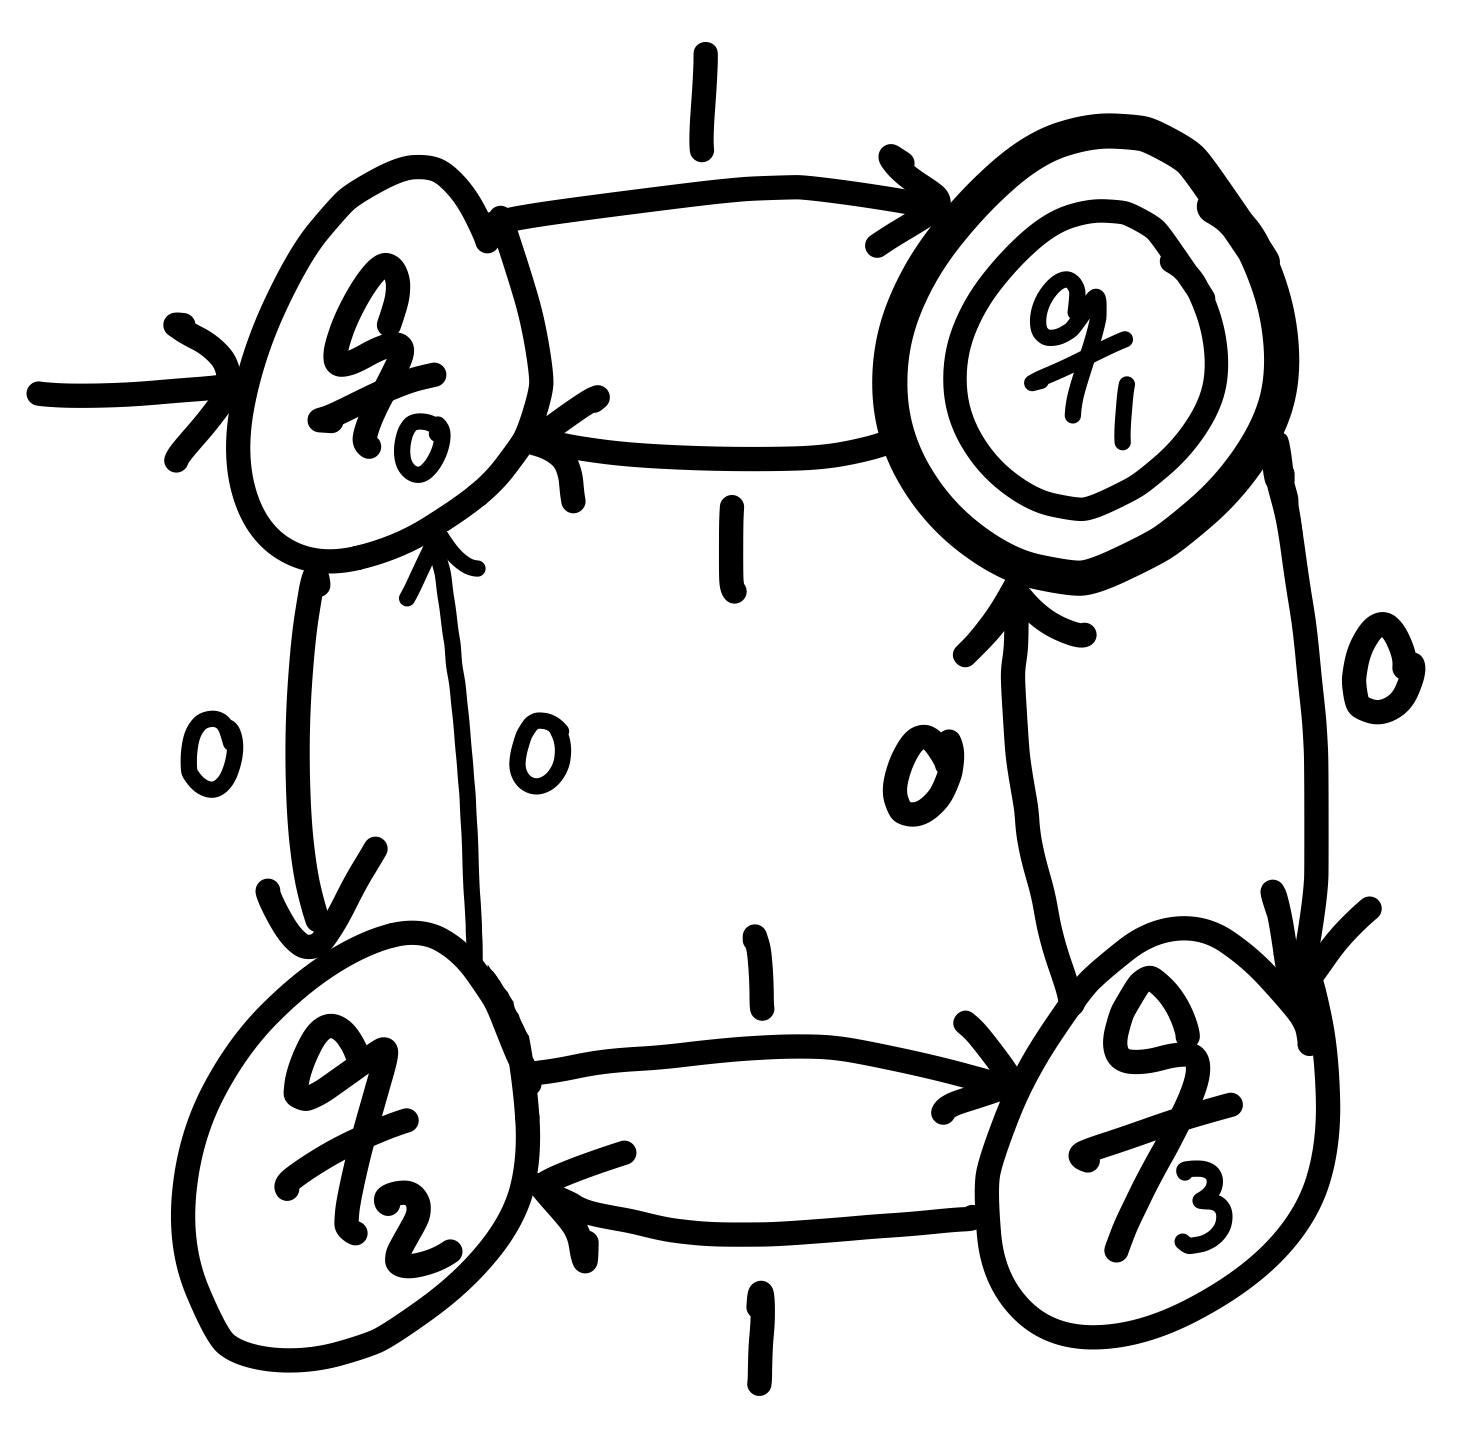
\includegraphics[scale=0.2]{2.8}


            2.12. $\left\{w \in\{0,1\}^*:\right.$ the third character in $w$ is 0$\}$


            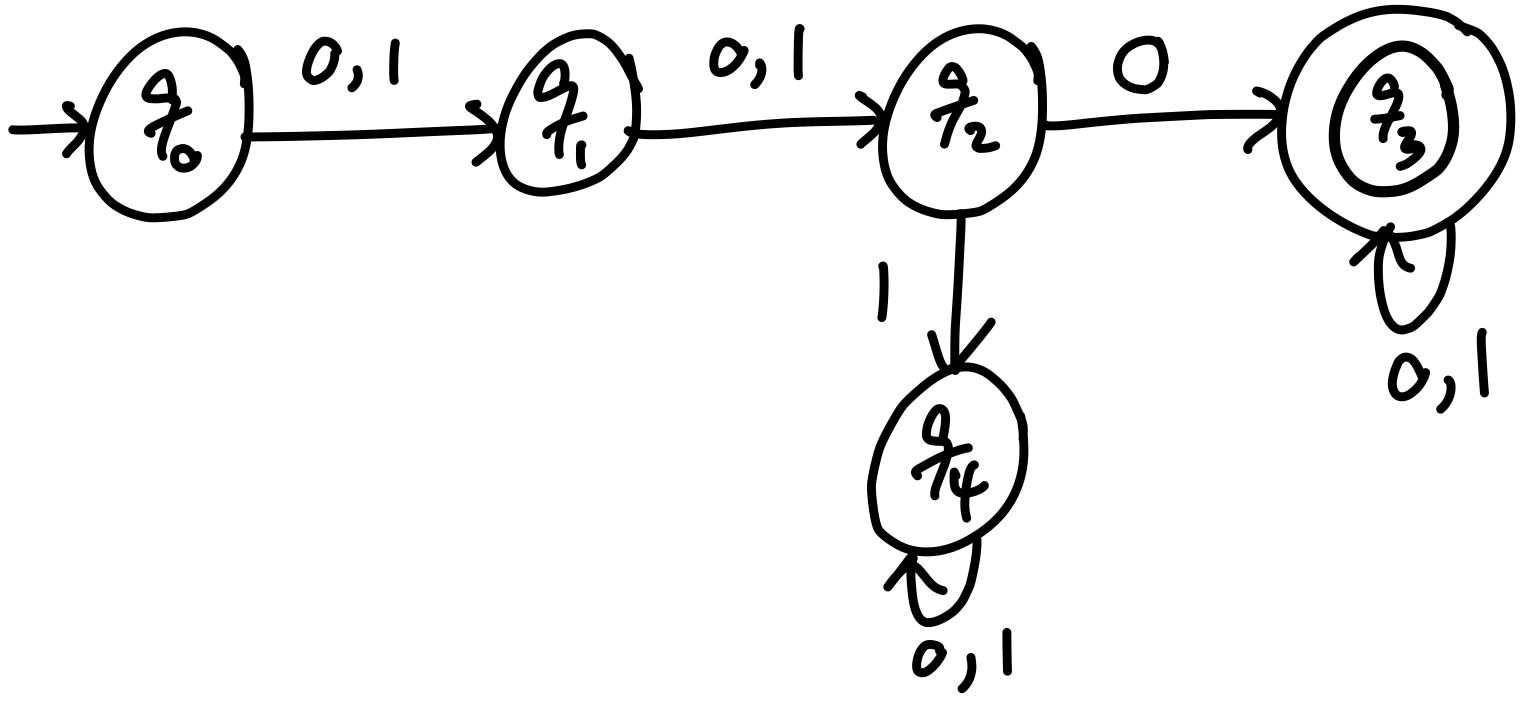
\includegraphics[scale=0.2]{2.12}


            2.14. $\left\{w \in\{0,1\}^*: w\right.$ starts or ends with a 0$\}$


            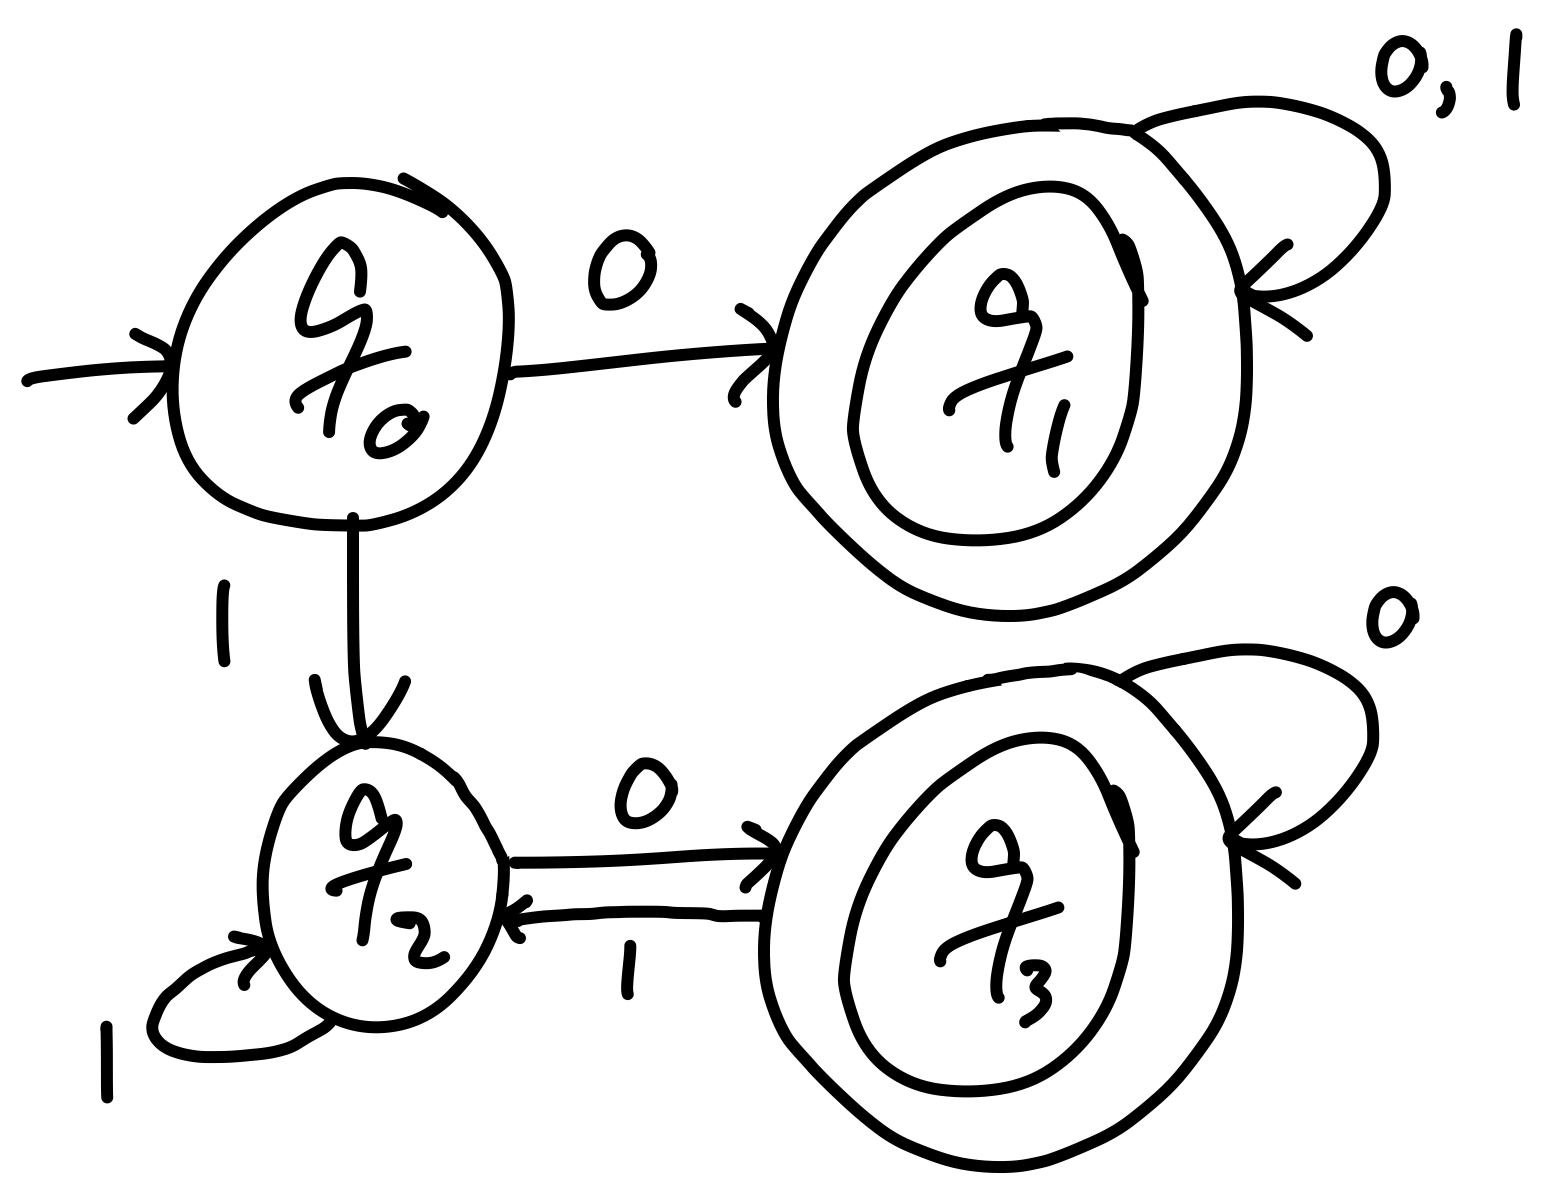
\includegraphics[scale=0.2]{2.14}


            2.15. $\left\{w \in\{0,1\}^*: w\right.$ has exactly one 0$\}$


            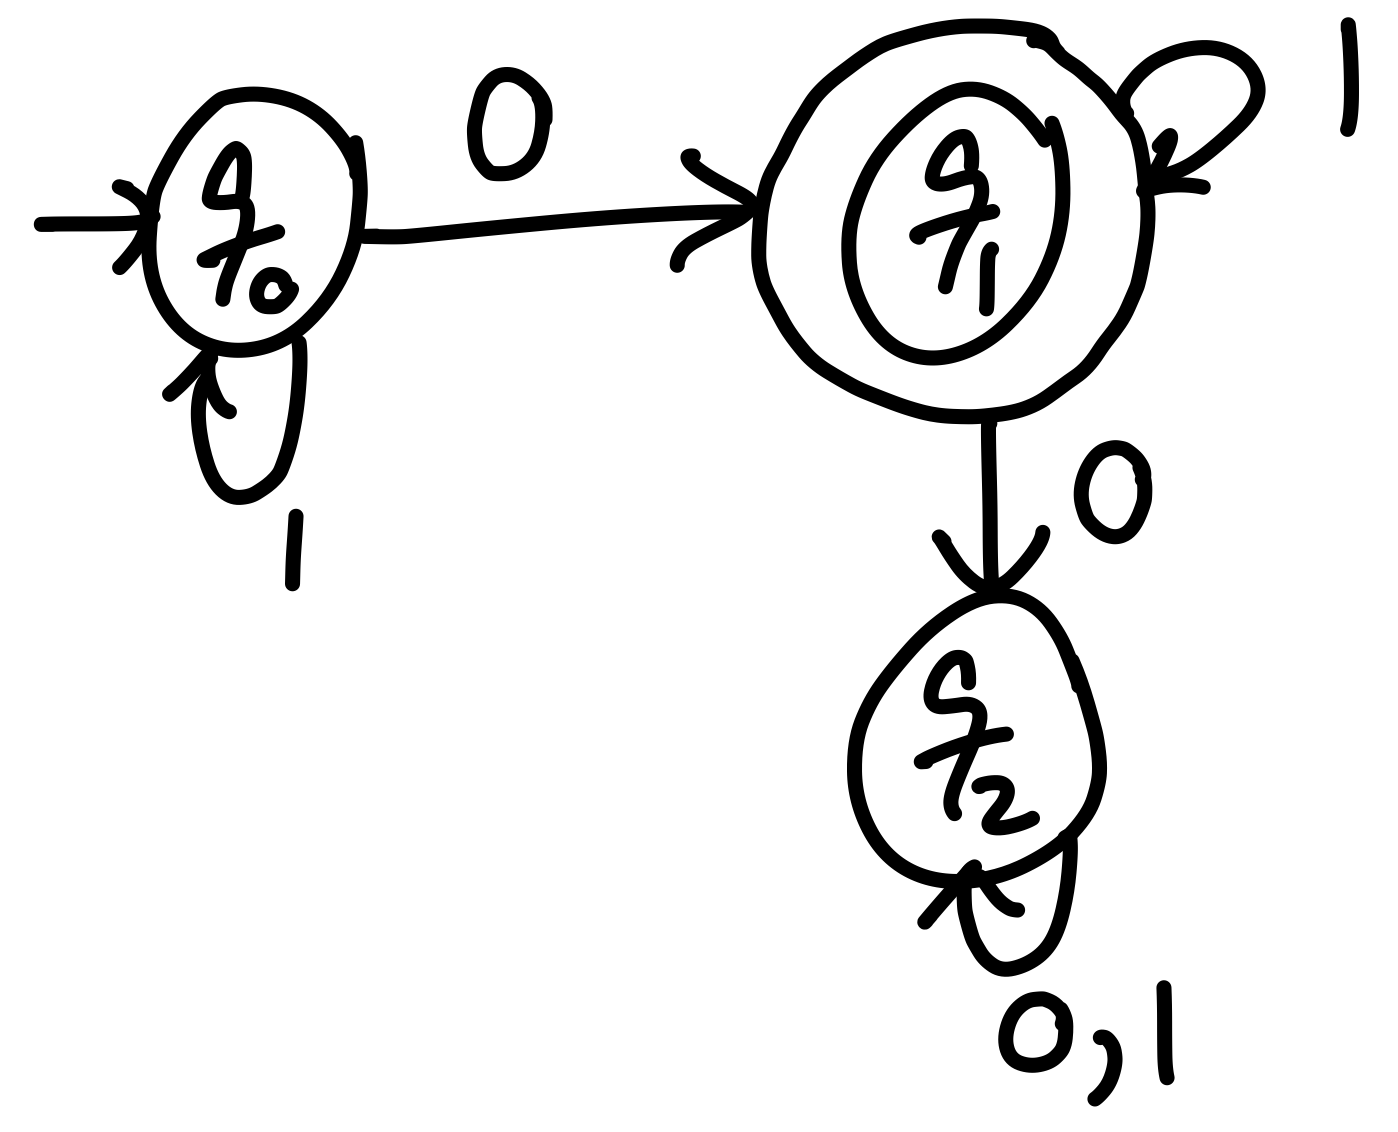
\includegraphics[scale=0.2]{2.15}


            2.16. $\left\{w \in\{0,1\}^*: w\right.$ contains 10 but not 1010$\}$


            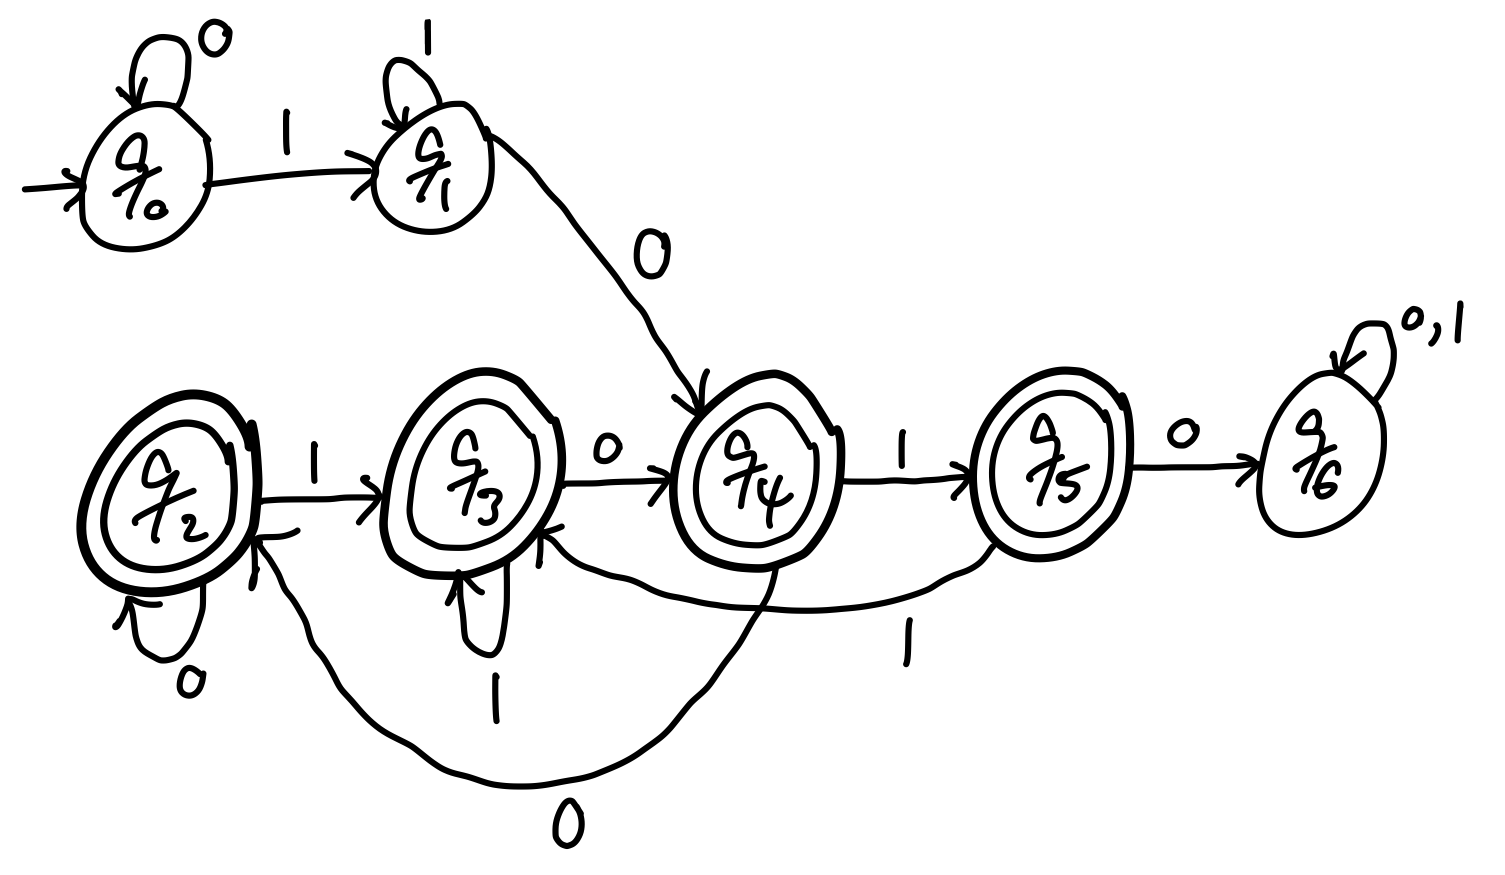
\includegraphics[scale=0.2]{2.16}


            2.18. $\left\{w \in\{0,1\}^*: w\right.$ contains at most two 0s and at least one 1$\}$


            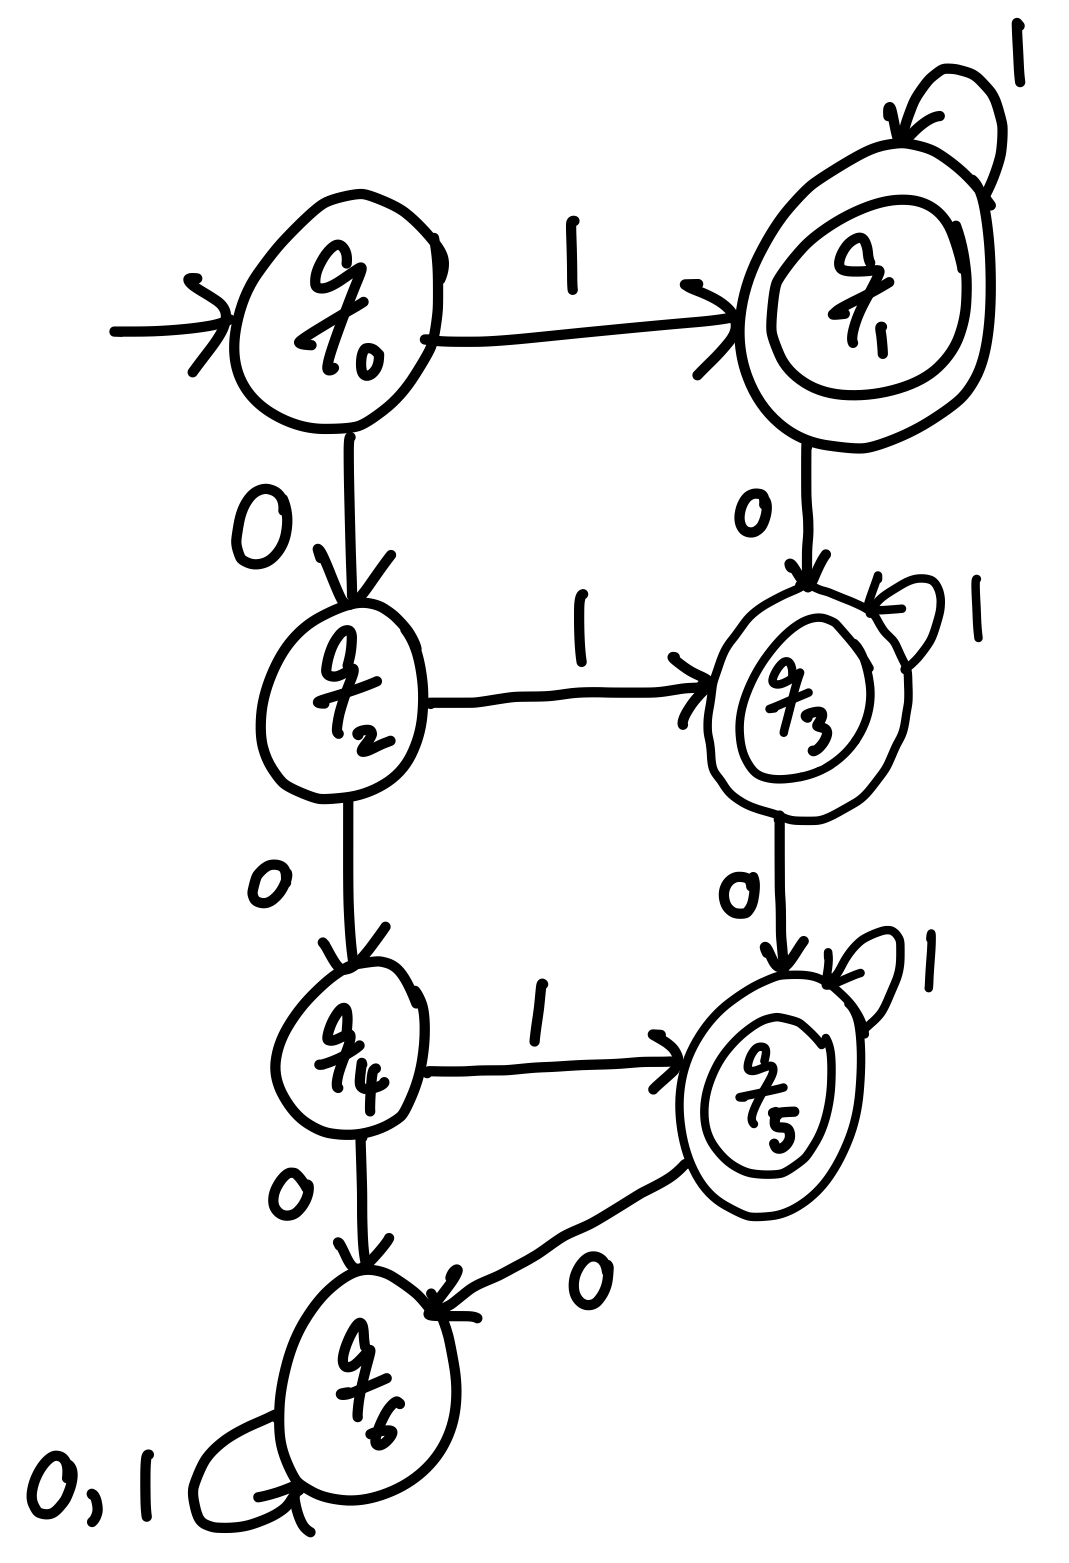
\includegraphics[scale=0.2]{2.18}


            2.19. $\left\{w \in\{0,1\}^*:\right.$ the number of 0s in $w$ is divisble by 3$\}$


            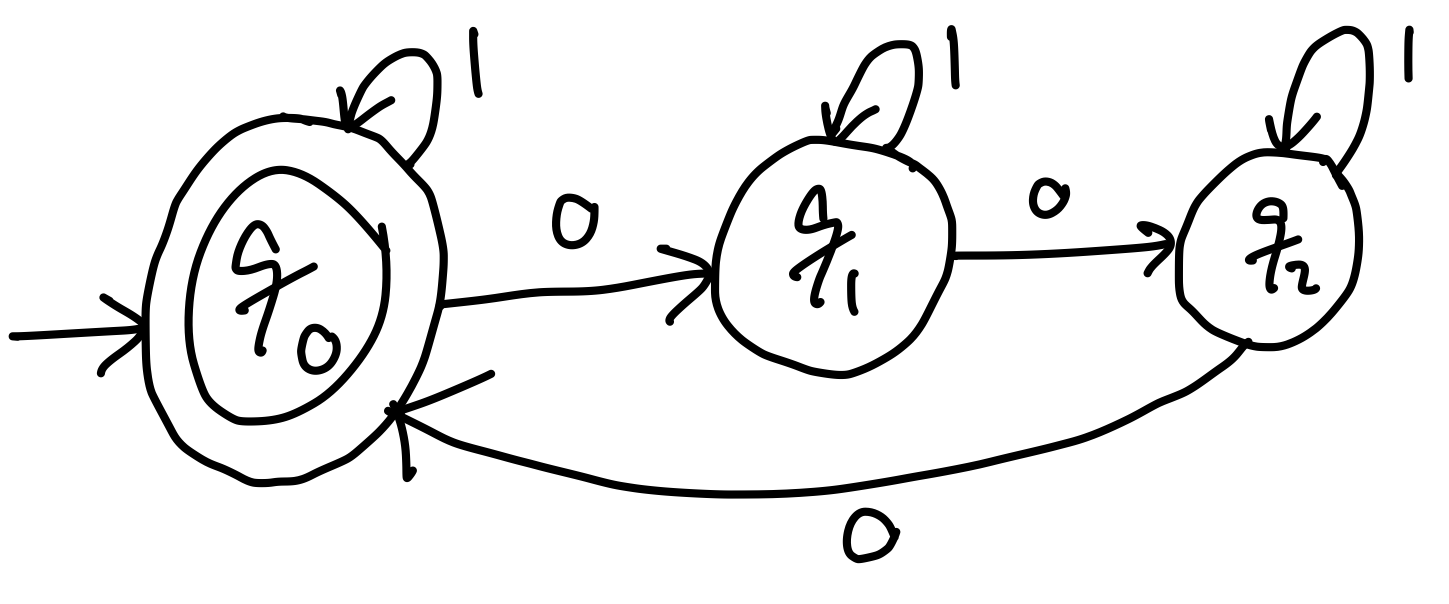
\includegraphics[scale=0.2]{2.19}


            2.24. $\left\{w \in\{0, \ldots, 9\}^*: w\right.$ is divisible by 5 in decimal $\}$ (Let $\lambda$ be in the language and ignore leading 0s.)


            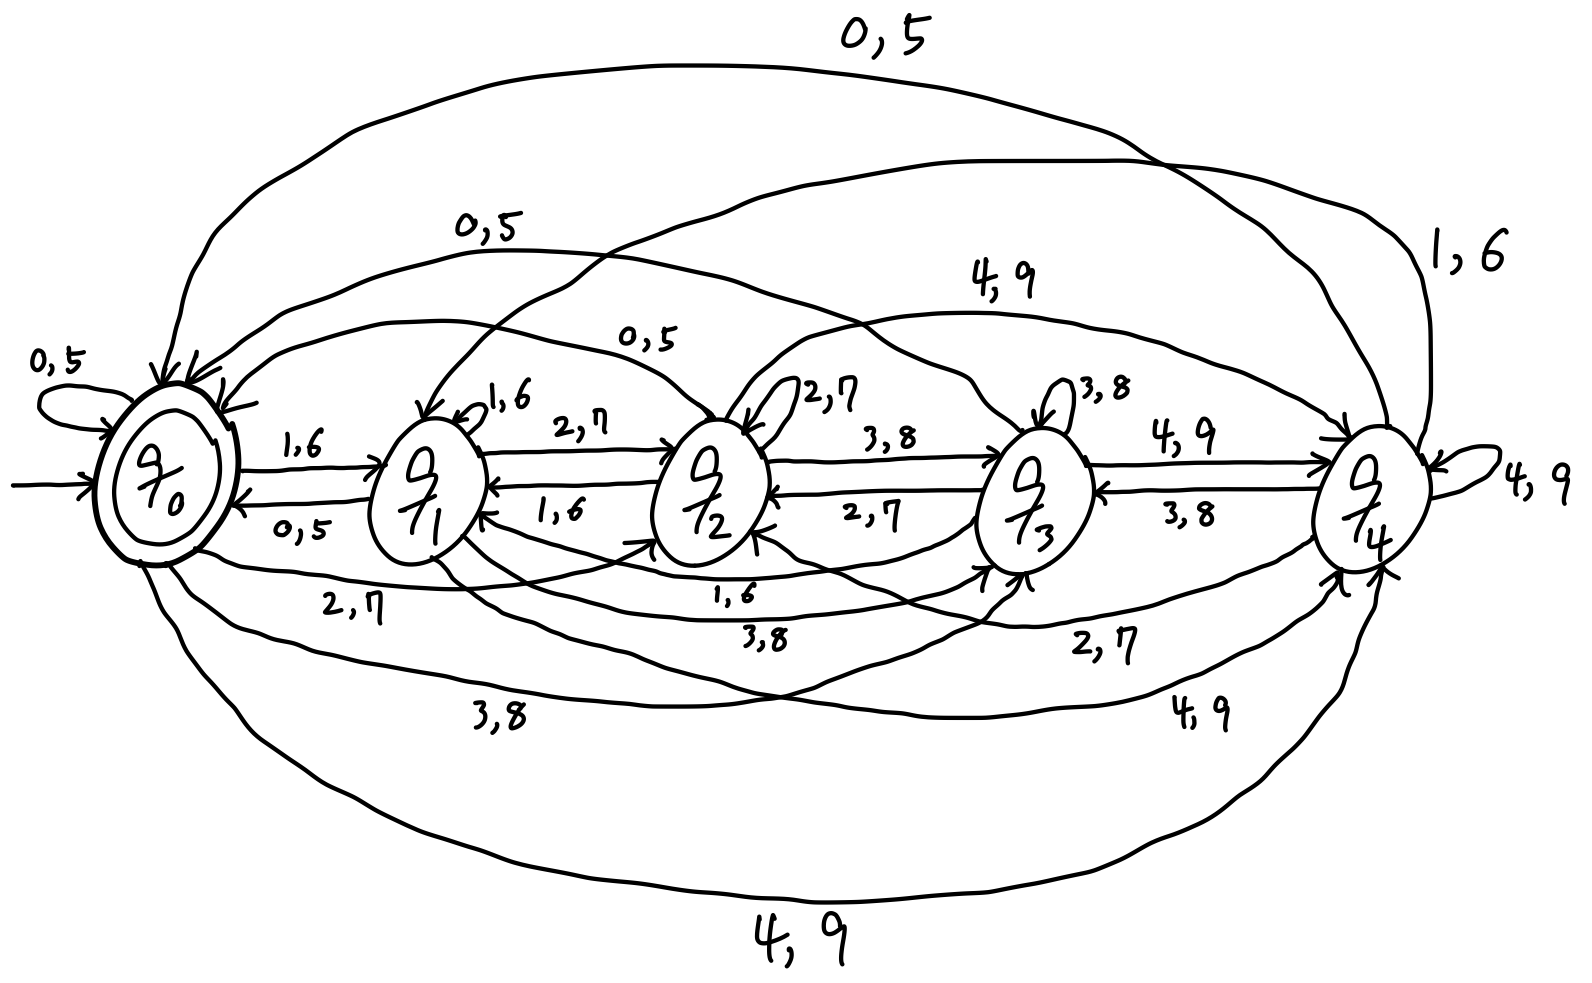
\includegraphics[scale=0.2]{2.24}


            2.27. $\left\{w \in\{A, C, G, T\}^*: w\right.$ has the substring ATG followed later by the substring TAA or TAG or TGA $\}$


            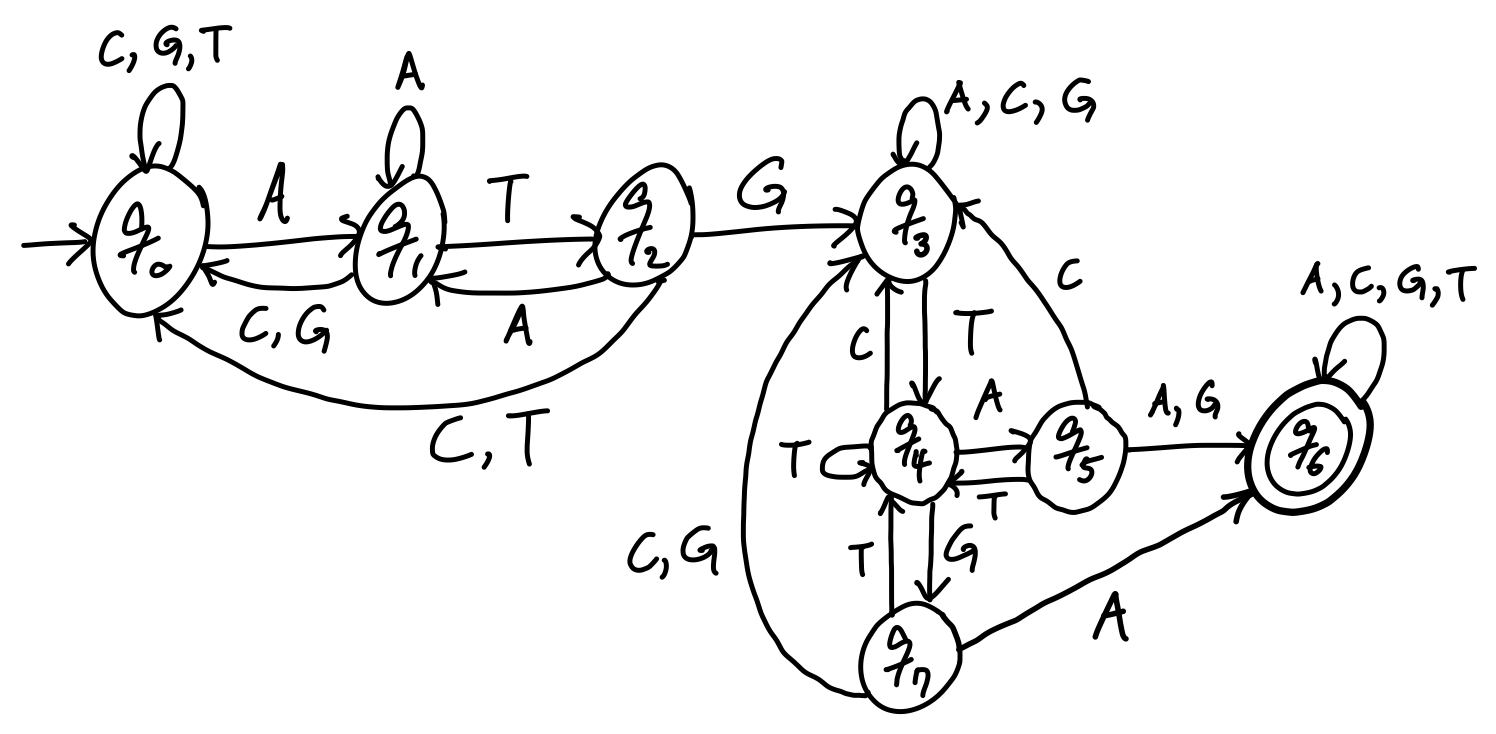
\includegraphics[scale=0.2]{2.27}



      \item Determine whether each of the following statements is true or false. Give a one line explanation for each.


            3.4. (Assume that $x = 3$) $(x \leq 3) \vee(x \leq 2)$

            True. The above statement's value is true if  either $(x \leq 3)$ or $(x \leq 2)$ is true and the given assumption makes the statement $(x \leq 3)$ to true.


            3.5. (Assume that $x = 3$ and $y=4$) $(x<y) \wedge(x+1 \leq y)$

            True. Based on the given assumption, the statement $(x<y)$ is true and also $(x+1 \leq y)$ is true, which the conjunction's value that is based on these two statement results true.


      \item Write each of the following statements in symbolic form in terms of $\lnot $, $\wedge$, and $\vee$ operations

            3.13. The value $x$ is smaller than zero or at least eleven.

            $(x < 0) \vee (x \geq 11)$

            3.19. Exactly two of the values $x, y, z$ are equal to ten.

            $(x=10 \wedge y=10 \wedge \lnot(z=10)) \vee (x=10 \wedge \lnot(y = 10) \wedge z=10) \vee (\lnot(x=10) \wedge y=10 \wedge z=10)$

      \item Show whether the following pairs of expressions are equivalent by creating truth
            tables for them. Be sure to show each of the intermediate steps for each expression.

            3.27. $A \wedge(A \vee B)$ and $A$


            \begin{tabular}{ |c|c|c|c|  }
                  \hline
                  $A$ & $B$ & $A \vee B$ & $A \wedge(A \vee B)$ \\
                  \hline
                  F   & F   & F          & F                    \\
                  F   & T   & T          & F                    \\
                  T   & F   & T          & T                    \\
                  T   & T   & T          & T                    \\
                  \hline
            \end{tabular}


            3.33. $A \vee(B \wedge C)$ and $(A \vee B) \wedge(A \vee C)$

            \begin{tabular}{ |c|c|c|c|c|c|c|c|  }
                  \hline
                  $A$ & $B$ & $C$ & $A \vee B$ & $A \vee C$ & $B \wedge C$ & $A \vee(B \wedge C)$ & $(A \vee B) \wedge(A \vee C)$ \\
                  \hline
                  F   & F   & F   & F          & F          & F            & F                    & F                             \\
                  F   & F   & T   & F          & T          & F            & F                    & F                             \\
                  F   & T   & F   & T          & F          & F            & F                    & F                             \\
                  F   & T   & T   & T          & T          & T            & T                    & T                             \\
                  T   & F   & F   & T          & T          & F            & T                    & T                             \\
                  T   & F   & T   & T          & T          & F            & T                    & T                             \\
                  T   & T   & F   & T          & T          & F            & T                    & T                             \\
                  T   & T   & T   & T          & T          & T            & T                    & T                             \\
                  \hline
            \end{tabular}

      \item Write each of the following statements in the form $P \Rightarrow Q$ or $P \Leftrightarrow Q$, stating the values of $P$ and $Q$ for each.

            3.36. The sum of two numbers is an integer if both numbers are integers.

            $P$: Both numbers are integers.

            $Q$: The sum of two numbers is an integer.

            $P \Rightarrow Q$


            3.38. It is safe to divide by $x$ only if $x \neq 0$.

            $P$: It is safe to divide by $x$.

            $Q$: $x \neq 0$

            $P \Rightarrow Q$

      \item Show whether the following pairs of expressions are equivalent by creating truth
            tables for them. Be sure to show each of the intermediate steps for each expression.


            3.40. $A \vee B$ and $\neg A \Rightarrow B$

            \begin{tabular}{ |c|c|c|c|c|  }
                  \hline
                  $A$ & $B$ & $\neg A$ & $A \vee B$ & $\neg A \Rightarrow B$ \\
                  \hline
                  F   & F   & T        & F          & F                      \\
                  F   & T   & T        & T          & T                      \\
                  T   & F   & F        & T          & T                      \\
                  T   & T   & F        & T          & T                      \\
                  \hline
            \end{tabular}


            3.41. $A \wedge B$ and $A \Rightarrow \neg B$

            \begin{tabular}{ |c|c|c|c|c|  }
                  \hline
                  $A$ & $B$ & $\neg B$ & $A \wedge B$ & $A \Rightarrow \neg B$ \\
                  \hline
                  F   & F   & T        & F            & T                      \\
                  F   & T   & F        & F            & T                      \\
                  T   & F   & T        & F            & T                      \\
                  T   & T   & F        & T            & F                      \\
                  \hline
            \end{tabular}


            3.42. $A \Leftrightarrow B$ and $(\neg A \vee B) \wedge(A \vee \neg B)$


            \begin{tabular}{ |c|c|c|c|c|c|c|c|  }
                  \hline
                  $A$ & $B$ & $\neg A$ & $\neg B$ & $\neg A \vee B$ & $A \vee \neg B$ & $(\neg A \vee B) \wedge(A \vee \neg B)$ & $A \Leftrightarrow B$ \\
                  \hline
                  F   & F   & T        & T        & T               & T               & T                                       & T                     \\
                  F   & T   & T        & F        & T               & F               & F                                       & F                     \\
                  T   & F   & F        & T        & F               & T               & F                                       & F                     \\
                  T   & T   & F        & F        & T               & T               & T                                       & T                     \\
                  \hline
            \end{tabular}


            3.44. $(A \Rightarrow B) \vee(A \Rightarrow C)$ and $A \Rightarrow(B \vee C)$


            \begin{tabular}{ |c|c|c|c|c|c|c|c|  }
                  \hline
                  $A$ & $B$ & $C$ & $A \Rightarrow B$ & $A \Rightarrow C$ & $B \vee C$ & $(A \Rightarrow B) \vee(A \Rightarrow C)$ & $A \Rightarrow(B \vee C)$ \\
                  \hline
                  F   & F   & F   & T                 & T                 & F          & T                                         & T                         \\
                  F   & F   & T   & T                 & T                 & T          & T                                         & T                         \\
                  F   & T   & F   & T                 & T                 & T          & T                                         & T                         \\
                  F   & T   & T   & T                 & T                 & T          & T                                         & T                         \\
                  T   & F   & F   & F                 & F                 & F          & F                                         & F                         \\
                  T   & F   & T   & F                 & T                 & T          & T                                         & T                         \\
                  T   & T   & F   & T                 & F                 & T          & T                                         & T                         \\
                  T   & T   & T   & T                 & T                 & T          & T                                         & T                         \\
                  \hline
            \end{tabular}


            3.46. $(A \Rightarrow C) \wedge(B \Rightarrow C)$ and $(A \vee B) \Rightarrow C$


            \begin{tabular}{ |c|c|c|c|c|c|c|c|  }
                  \hline
                  $A$ & $B$ & $C$ & $A \Rightarrow C$ & $B \Rightarrow C$ & $A \vee B$ & $(A \Rightarrow C) \wedge(B \Rightarrow C)$ & $(A \vee B) \Rightarrow C$ \\
                  \hline
                  F   & F   & F   & T                 & T                 & F          & T                                           & T                          \\
                  F   & F   & T   & T                 & T                 & F          & T                                           & T                          \\
                  F   & T   & F   & T                 & F                 & T          & F                                           & F                          \\
                  F   & T   & T   & T                 & T                 & T          & T                                           & T                          \\
                  T   & F   & F   & F                 & T                 & T          & F                                           & F                          \\
                  T   & F   & T   & T                 & T                 & T          & T                                           & T                          \\
                  T   & T   & F   & F                 & F                 & T          & F                                           & F                          \\
                  T   & T   & T   & T                 & T                 & T          & T                                           & T                          \\
                  \hline
            \end{tabular}

\end{enumerate}

\end{document}